\documentclass[9pt]{extarticle}

\usepackage[utf8]{inputenc}              % Tipos de caracteres
\usepackage[portuguese]{babel}           % Português
\usepackage[a4paper,portrait]{geometry}  % Tipo de papel
\usepackage{color}                       % Para tratamento da cor
\usepackage{graphicx}                    % Para a imagem
\DeclareGraphicsExtensions{.jpg,.png}
\usepackage{amsmath}                     % Para as matematiquices
\usepackage{amssymb}
\usepackage{array}
\usepackage{gensymb}                     % Grau
\usepackage{multicol}
\setlength{\columnsep}{1cm}
\usepackage{geometry}					% Margens
%\usepackage{xfrac}
\usepackage{colortbl}

\usepackage{multirow}

\addtolength{\topmargin}{-20mm}
\addtolength{\textheight}{55mm}
\addtolength{\oddsidemargin}{-15mm}
\addtolength{\textwidth}{32mm}

\renewenvironment{abstract}
 {\small
  \begin{center}
  \bfseries \abstractname\vspace{-.5em}\vspace{0pt}
  \end{center}
  \list{}{
    \setlength{\leftmargin}{0cm}%
    \setlength{\rightmargin}{\leftmargin}%
  }%
  \item\relax}
 {\endlist}
 
\renewcommand{\abstractname}{Resumo}
%\renewcommand{\bibname}{Referências}

\delimitershortfall-1sp
\newcommand\abs[1]{\left|#1\right|}
\newcommand{\PR}[1]{\ensuremath{\left[#1\right]}}
\newcommand{\PC}[1]{\ensuremath{\left(#1\right)}}
\newcommand{\chav}[1]{\ensuremath{\left\{#1\right\}}}

\newcolumntype{x}[1]{>{\centering\hspace{0pt}}p{#1}}

\begin{document}

\title {\bf \huge T1 - Conversor Termoelétrico}
\author
{{\small Grupo III - João Ferreira (78179) Henrique Rodrigues (78632) Rodrigo C. Carvalho (78646) Cristina Melício (78947)} \\
{\small MEFT - 2ºAno, 2º Semestre - Laboratório de Complementos de Eletromagnetismo e Termodinâmica}}
\date{{\small Sexta-Feira, 13 de Março de 2015}}
\maketitle

\begin{abstract}

\end{abstract}

\begin{multicols}{2}

\section{Introdução}

\par O objetivo deste trabalho experimental é o estudo dum dos fenómenos de transferência de calor - a condução - e a consequente determinação do coeficiente de condutividade do alumínio. 

\par A condução de calor ou condução térmica é um fenómeno de transferência de energia interna entre corpos em contacto, sem trocas de massa e que ocorre devido à existência de um gradiente de temperatura no meio. O calor transferido por um corpo por unidade de tempo é dado pela expressão:

\begin{equation} \label{calor}
\frac{dQ}{dt} = \rho c \frac{dT}{dt} dV
\end{equation}
\begin{center}
\par\noindent {\scriptsize(onde que $\rho$ é a densidade do material e $c$ o seu calor específico)}
\end{center}

Este fenómeno pode ser modelado através da Lei de Fourier que estabelece uma relação linear entre o fluxo local de calor $\vec{j_Q}$ e o simétrico do gradiente de temperatura $\nabla\vec{T}$, cuja expressão é:

\begin{equation}
\vec{j_Q} = - k \nabla\vec{T}
\end{equation}
\begin{center}
\par\noindent {\scriptsize(em que $k$ é o coeficiente de condutividade térmica do material)}
\end{center}

Integrando a equação anterior sobre uma superfície arbitrária fechada $S$ e aplicando o Teorema da Divergência obtém-se:

\begin{equation} \label{3}
\frac{\partial Q}{\partial t} = \oint_S (\vec{j_Q} \cdot \vec{n}) \,dS = \int_V - k \nabla^2 \vec{T} \,dV
\end{equation}

Por outro lado, integrando a equação \label{calor} tem-se:
\begin{equation} \label{4}
\frac{\partial Q}{\partial t} = - \int_V \rho c \frac{\partial T}{\partial t} \,dV
\end{equation}

Igualando as expressões dentro do integral de \ref{3} e \ref{4} resulta a Equação do Calor:
\begin{equation}
\frac{\partial T}{\partial t} = \chi \nabla^2 T 
\end{equation}
\begin{center}
\par\noindent {\scriptsize(em que $\chi = \frac{k}{\rho c}$ é a difusividade e $\nabla^2 T$ o Laplaciano da temperatura)}
\end{center}

\subsection*{Regime Estacionário}
\par Designa-se por regime estacionário a situação em que a temperatura não depende do tempo, ou seja $\frac{\partial T}{\partial t} = 0 \Rightarrow \vec{T}(\vec{r},t) \equiv \vec{T}(\vec{r})$.
\par Considera-se então, uma barra de alumínio de secção de área $S$ e comprimento $l$, em contacto com duas fontes de temperatura nas suas extremidades e o resto isolado, de modo a que, o seu fluxo possa ser visto como unidimensional, isto é, $\vec{T}(r) \equiv \vec{T}(x)$.
\begin{equation}
\nabla^2 T = 0 \Leftrightarrow \frac{\partial ^2 T}{\partial x^2} = 0 \Rightarrow \frac{\partial T}{\partial x} = c_1 \Rightarrow T(x) = c_1 x + c_2
\end{equation}

Impondo as condições fronteira $T(0) = T_{Q}$ e $T(l) = T_{F}$ obtém-se a expressão para a temperatura em função da posição na barra: 
\begin{equation}
T(x) = \frac{T_ {Q} - T_{F}}{l}x + T_{Q}
\end{equation}

Por fim, a fórmula para a condutividade de um material é dada por:
\begin{equation}
k = \frac{\frac{dQ}{dt}}{S|\frac{dT}{dx}|}
\end{equation}
\begin{center}
\par\noindent {\scriptsize(onde $S$ é a superfície lateral por onde a potência flui)}
\end{center}

\subsection*{Regime Variável}
Neste caso, tem-se também que o fluxo pode ser visto como unidimensional, no entanto considera-se que existe variação da temperatura com o tempo, logo $\frac{\partial T}{\partial t} \neq 0$, e por isso, fica-se com  $\vec{T}(\vec{r},t) \equiv \vec{T}(x,t)$.

\par Para resolver a Equação do Calor nesta situação impõe-se as condições fronteira $T(0,t) = T_{Q}$ e $T(l,t) = T_{F}$ e condição inicial $T(x,0) = \frac{T_{Q} - T_{F}}{l} + T_{Q}$. Com o auxilio da análise de Fourier obtém-se a expressão para a temperatura seguinte:

\begin{eqnarray}
\begin{split}
& T(x,t)= T_{F} + (T_{Q} - T_{F})\frac{8}{\pi ^2}\sum_{n=0}^{n} e^{-\frac{\chi}{L^2}(\frac{\pi}{2} + n\pi)^2 t}  \frac{(-1)^n}{(2n+1)^2} \\
&\sin \left(\frac{x}{L}\left(\frac{\pi}{2} + n\pi \right)\right)
\end{split}
\end{eqnarray}

\section{Montagem da Experiência}

\par A montagem experimental para esta experiência consiste numa barra de alumínio, com uma extremidade em contacto com uma fonte quente e a outra a uma fonte fria, estando estas três partes termicamente isoladas.
\par A barra tem $12cm$ de comprimento e uma secção de $4cm^2$ e, ao longo da mesma, existem 5 sensores de temperatura. Estes sensores estão ligados a um computador que possui um software especializado de aquisição de dados, que permite a visualização dos valores de temperatura em tempo real.

\subsection*{Regime Estacionário}
Para a primeira parte o diagrama da montagem experimental encontra-se na figura 1. 

\begin{center}
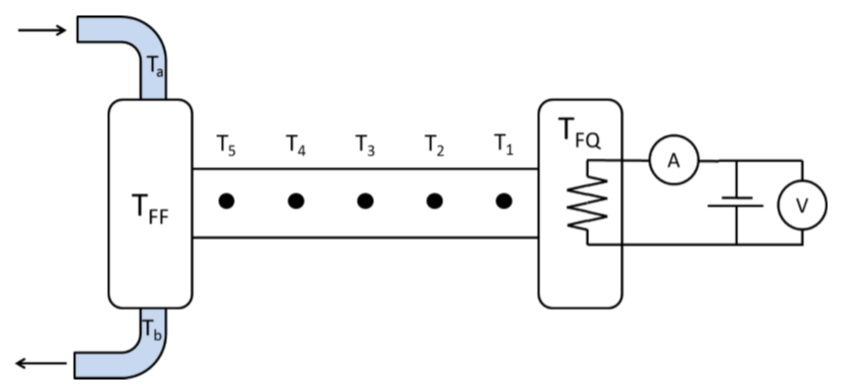
\includegraphics[width=160pt]{figura1.jpg}
\par\noindent {\scriptsize (Figura 1: Esquema da montagem para o regime estacionário)}
\end{center}

\par A fonte quente é constituída por um circuito resistivo ligado a uma placa de cobre em contacto com a barra, sendo alimentado por uma fonte de tensão. A tensão e a corrente que percorrem a resistência podem ser determinadas através de um voltímetro e um amperímetro, sendo a potência fornecida à placa dada pela Lei de Joule:
\begin{equation}
P_Q = U I
\end{equation}
\par A fonte fria é constituída por um sistema de refrigeração com água cuja temperatura à entrada e a saída é $T_a$ e $T_b$, respetivamente. Sendo assim, a potência fornecida pela fonte pode ser determinada pela equação \ref{PF}, em que $\phi$ é o caudal calculado pela expressão \ref{caudal}.
\begin{equation}\label{PF}
P_F = c \phi (T_b - T_a)
\end{equation}
\begin{equation} \label{caudal}
\phi = \frac{V_\rho}{\Delta t}
\end{equation}

\subsection*{Regime Variável}
Para a segunda parte considera-se o esquema da montagem experimental da figura 2, em que foi retirado o sistema de aquecimento, estando a barra apenas em contacto com o sistema de arrefecimento.

\begin{center}
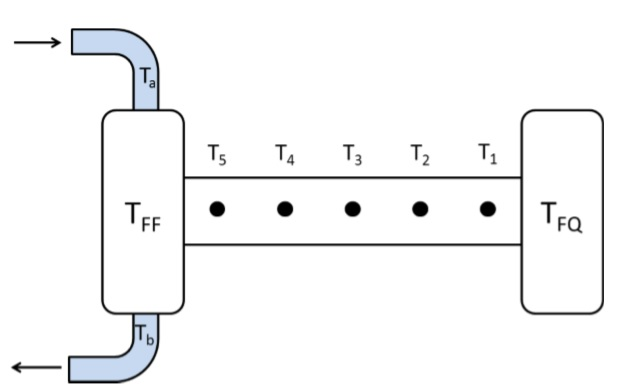
\includegraphics[width=140pt]{figura2.jpg}
\par\noindent {\scriptsize (Figura 2: Esquema da montagem para o regime variável)}
\end{center}







\begin{thebibliography}{9}

\bibitem{guia} Guia de objetivos do trabalho, Professor João Figueirinhas
\bibitem{apontamentos} Apontamentos das aulas teóricas
%\bibitem{site} Wikipedia, the free encyclopedia - Thermoelectric effect. [Online] Available from: \url{http://en.wikipedia.org/wiki/thermoelectric\_effect}
\end{thebibliography}

\vfill

\pagebreak

%\section{Anexos}
%\subsection*{\normalsize Material}
%\begin{itemize}
%\item Cenas
%\end{itemize}
%
%\subsection*{\normalsize Tabelas Completas de Resultados}
%\par Cenas

\end{multicols}

\end{document}

% FOTOGRAFIA
%\begin{center}
%\includegraphics[width=240pt]{NOME SEM EXTENSAO}
%\par\noindent {\scriptsize (Figura X: Descrição)}
%\end{center}

%NOVA SUBSECÇÃO
%\subsection*{\normalsize BLA BLA}

%TABELA
%\begin{center}
%\begin{tabular}{ x{1.5cm} ... }
%i & ... \tabularnewline
%\hline \hline
%1 & 4.15  & 0.15  & 2033 & -  \tabularnewline
%\end{tabular}
%\par\noindent {\scriptsize (Tabela X: Descrição)}
%\end{center}